\def\year{2019}\relax
%File: formatting-instruction.tex
\documentclass[letterpaper]{article} %DO NOT CHANGE THIS
%\newcommand{\CLASSINPUTbaselinestretch}{1.2}
%\documentclass[conference,twocolumn]{IEEEtran}
%\documentclass[letterpaper,10 pt,conference]{ieeeconf} 
%\documentclass[10pt, onecolumn]{IEEEtran}
%\documentclass[10pt,letterpaper]{article}
%\IEEEoverridecommandlockouts    
% \overrideIEEEmargins


%\usepackage[left=1in,top=1in,right=1in,bottom=1in]{geometry}


% \usepackage{geometry}
% \geometry{
% a4paper,
% total={210mm,297mm},
% left=17.1mm,
% right=17.1mm,
% top=19.1mm,
% bottom=17.1mm,
% }


\usepackage[english]{babel}
\usepackage{enumitem, hyperref}
\usepackage[latin1]{inputenc}
\usepackage{enumerate}
%\usepackage{enumitem}
%\setlist[enumerate]{label=\roman*}  %% for all enumerate environments
\usepackage{graphicx}
\usepackage{color}
\usepackage[dvipsnames]{xcolor}
\usepackage[T1]{fontenc}
\usepackage{subfigure}
%\usepackage{subcaption}
\usepackage{dsfont}
\usepackage{amsfonts}
\usepackage{graphicx,wrapfig}
\usepackage[T1]{fontenc}
\usepackage{amsmath}
\usepackage{mathtools, cuted}
\usepackage{amsthm}
\usepackage{amstext}
\usepackage{amssymb}
\usepackage{mathrsfs}
%\usepackage{cite}
\usepackage{mathtools}
\usepackage{tikz}
\usepackage{marginnote}
\usepackage{tkz-tab}
\usetikzlibrary{topaths,calc}
%*****Margin Note
\usepackage{stackengine}

%**********

\newcommand{\appsec}{
	\renewcommand{\thesubsection}{\Alph{subsection}}
}
\def\R{\mathbb{R}}
\def\cE{\mathcal{E}}
\def\fin{{<\infty}}
\def\supp{\mathop{\rm supp}}
\def\Gr{\mathop{\rm Gr}}
\def\cl{\mathop{\rm cl}}
\def\Proj{\mathop{\rm Proj}}
\def\argmax{\mathop{\rm arg\, max}}
\def\argmin{\mathop{\rm arg\, min}}
\def\eps{\varepsilon}
\def\hX{\hat{X}}
\def\hY{\hat{Y}}
\def\hx{\hat{x}}
\def\hf{\hat{f}}
\def\A{{\mathcal A}}
\def\B{{\mathcal B}}
\def\D{{\mathcal D}}
\def\F{{\mathcal F}}
\def\H{{\mathcal H}}
\def\I{{\mathcal I}}
\def\G{{\mathcal G}}
\def\C{{\mathcal C}}
\def\P{{\mathcal P}}
\def\Q{{\mathcal Q}}
\def\T{{\mathcal T}}
\def\X{{\mathcal X}}
\def\Y{{\mathcal Y}}
\def\M{{\mathcal M}}
\def\N{{\mathcal N}}
\def\S{{\mathcal S}}
\def\L{{\mathcal L}}
\def\cR{{\mathcal R}}
\def\Z{{\mathcal Z}}
\def\U{{\mathcal U}}
\def\V{{\mathcal V}}
%\newcommand{\indep}{\perp\!\!\!\perp}
\def\indep{{\perp\!\!\!\perp}}
\def\sgr{{\mathsf{gr}}}
\def\spr{{\mathsf{pr}}}
\def\sPr{{\mathsf{Pr}}}
\def\sUnif{{\mathsf{Unif}}}
\def\sBer{{\mathsf{Bernoulli}}}
\def\sP  {{\mathsf{P}}}
\def\sp{{\mathsf p}}
\def\sq{{\mathsf q}}
\def\sX{{\mathsf X}}
\def\sY{{\mathsf Y}}
\def\sZ{{\mathsf Z}}
\def\sM{{\mathsf {sENSR}}}
\def\sE{{\mathsf E}}
\def\sF{{\mathsf F}}
\def\sU{{\mathsf U}}
\def\sV{{\mathsf V}}
\def\sW{{\mathsf {W}}}
\def\sG{{\mathsf G}}
\def \var {{\mathsf {var}   }}
\def \mmse {{\mathsf {mmse}   }}
\def \cP {\mathsf{P}_{\mathsf{c}}}
\newcommand{\dsty}[1]{$\displaystyle #1$}
\def \AI {{I^{\mathsf{A}}}}
\def \nP {{\mathsf{P}^{(n)}}}
\def \np {{\mathsf{p}^{(n)}}}
\def \nq {{\mathsf{q}^{(n)}}}
\newcommand{\repdc}[3]{#1_{#2} , \ldots , #1_{#3}}
\usepackage[font=small,labelsep=space]{caption}
\captionsetup{%
	figurename=Fig.,
}
%\captionsetup{labelsep = }
\DeclareCaptionLabelSeparator{dot}{.~}
%\DeclareCaptionLabelSeparator{bar}{ | }
\captionsetup{
	labelsep=dot
}
%\theoremstyle{theorem}
%\theoremstyle{example}
\newcounter{example}
\newenvironment{example}[1][]{\refstepcounter{example}\par\medskip
	\noindent \textit{Example~\theexample. #1} \rmfamily}{\medskip}
%\newtheorem{example}{Example}
\newtheorem{definition}{Definition}
\newtheorem{theorem}{Theorem}
\newtheorem{corollary}{Corollary}
\newtheorem{fact}{Fact}
\newtheorem{proposition}{Proposition}
\newtheorem{lemma}{Lemma}
\theoremstyle{remark}
\newtheorem{remark}{Remark}
\newtheorem{conjecture}{Conjecture}
\newcommand{\markov}{\mathrel\multimap\joinrel\mathrel-%
	\mspace{-9mu}\joinrel\mathrel-}

\renewcommand{\qedsymbol}{\rule{0.5em}{0.5em}}
%%%%%%%%%%%%%%%%%%%%%%%%%%%%%%%%%%%%%%%%%%%%%%%%%%%%%%%%%%%%%%%%%%%%%%%%%%%%%%%%%%%%%%%%%55

\usepackage{times}
\usepackage{tikz}
\usepackage{amsmath}
\usepackage{verbatim}
\usetikzlibrary{arrows,shapes}
\tikzstyle{RectObject}=[rectangle,fill=white,draw,line width=0.2mm]
\tikzstyle{line}=[draw]
\tikzstyle{arrow}=[draw, -latex]
\usetikzlibrary{decorations.pathmorphing}
\usetikzlibrary{calc,shapes, positioning}
\usepackage{graphicx}
\usepackage{caption}
\usetikzlibrary{shapes.geometric}


\definecolor{DukeBlue}{HTML}{001A57}
\definecolor{DarkRed}{rgb}{0.75, 0.0, 0.0}
\definecolor{DarkGreen}{rgb}{0.0, 0.5, 0.0}
\newcommand{\TG}[1]{\textbf{\textcolor{DukeBlue}{(#1)}}}
\newcommand{\SK}[1]{\textbf{\textcolor{Magenta}{[#1]}}}
\newcommand{\md}[1]{\textcolor{Magenta}{#1}}



\DeclareFontFamily{U}{BOONDOX-calo}{\skewchar\font=45 }
\DeclareFontShape{U}{BOONDOX-calo}{m}{n}{
  <-> s*[1.05] BOONDOX-r-calo}{}
\DeclareFontShape{U}{BOONDOX-calo}{b}{n}{
  <-> s*[1.05] BOONDOX-b-calo}{}
\DeclareMathAlphabet{\mathcalboondox}{U}{BOONDOX-calo}{m}{n}
\SetMathAlphabet{\mathcalboondox}{bold}{U}{BOONDOX-calo}{b}{n}
\DeclareMathAlphabet{\mathbcalboondox}{U}{BOONDOX-calo}{b}{n}

%%%%%%%%%%%%%%%%%%%%%%%%%%%%%%%%%%%%%%%%%%%%%%%%%%%%%%%%%%%%%%%%%%%%%%%%%%%%%%%%%%%%%%%%5

% \IEEEoverridecommandlockouts

\allowdisplaybreaks

% Yi's delimiter
\newcommand{\paren}[1]{\left(#1\right)}
\newcommand{\set}[1]{\left\{#1\right\}}

\usepackage{aaai19}  %Required
\usepackage{times}  %Required
\usepackage{helvet}  %Required
\usepackage{courier}  %Required
\usepackage{url}  %Required
\usepackage{graphicx}  %Required
\frenchspacing  %Required
\setlength{\pdfpagewidth}{8.5in}  %Required
\setlength{\pdfpageheight}{11in}  %Required

%PDF Info Is Required:
\pdfinfo{
/Title (Wasserstein Soft Label Propagation on Hypergraphs: Algorithm and Generalization Error Bounds)
/Author (AAAI Press Staff)}
\setcounter{secnumdepth}{0}  

\begin{document}
% The file aaai.sty is the style file for AAAI Press 
% proceedings, working notes, and technical reports.
\title{Wasserstein Soft Label Propagation on Hypergraphs: Algorithm and Generalization Error Bounds}
\author{AAAI Press\\
Association for the Advancement of Artificial Intelligence\\
2275 East Bayshore Road, Suite 160\\
Palo Alto, California 94303\\
}
\maketitle

\begin{abstract}
Inspired by recent interests of developing machine learning and data mining algorithms on hypergraphs, we investigate in this paper the semi-supervised learning algorithm of propagating "soft labels" (e.g. probability distributions, class membership scores) over hypergraphs, by means of optimal transportation. Borrowing insights from Wasserstein propagation on graphs [Solomon et al. 2014], we re-formulate the label propagation procedure as message-passing algorithm, which renders itself naturally to a generalization applicable to hypergraphs through Wasserstein barycenters. Compared with Laplacian-based semi-supervised learning algorithms, the message-passing algorithm benefits from scalability and efficiency. Furthermore, in a PAC learning framework, we provide generalization error bounds for propagating one-dimensional distributions on graphs and hypergraphs using 2-Wasserstein distance, by establishing the \textit{algorithmic stability} of the proposed semi-supervised learning algorithm. These theoretical results also shed new lights upon deeper understandings of the Wasserstein propagation on graphs. We validate the efficacy of the proposed algorithm through a number of synthetic and real data experiments.
\end{abstract}
	
\section{Introduction}
In the last few decades, we have seen a significant progress in semi-supervised learning, a paradigm of statistical learning that leverages both labeled and unlabelled data. The main objective is to combine observed labels with the underlying graph/manifold structure of the dataset (e.g. the graph representation of dataset) to identify the labels for unlabelled data samples. We refer interested readers to \cite{Zhu06SSL} for

%\cite{Zhu06semi_supervisedlearning} for overviews of results. 

Given a dataset, it is a common practice to represent its manifold structure by a weighted graph $G=(V, E)$, where $V$ and $E$ correspond to data samples and their pairwise interactions, respectively. Let $f:V\to\D$ be an assignment of labels in an arbitrary set $\D$ to each vertex. Denote by $V_0\subset V$ the set of labelled vertices, that is $f(v)$ is known for all $v\in V_0$. The goal is to extend $f$ from $V_0$ to entire $V$. In the classical semi-supervised learning setup (e.g., see \cite{Zhu:SSL_Gaussian}) $\D$ is assumed to be a Euclidean space and hence the objective is formulated as minimizing the Dirichlet energy $\sum_{(u, v)\in E}(f(u)-f(v))^2$ over the space of functions $f$ satisfying the boundary condition on $V_0$. The labels are then given by a harmonic function satisfying $\Delta f=0$ on $V\backslash V_0$ for an appropriate positive definite Laplacian matrix $\Delta$.   

In many settings, however, it is natural to model the labels as histograms or probability distributions rather than numerical or categorical variables; we shall refer to these more general labels as \textit{soft} labels. For instance, the traffic density at a given router in the Internet network, or topic distributions in the co-authorship network, can be more naturally modeled as probability distributions. Soft labels not only generalize the numerical or categorical ``hard'' labels but also preserves more information of interest to real applications, such as the ``uncertainty'' of the estimation and inference. We model the assignment of soft labels to vertices as a distribution-valued map $V\to \D=\P(L)$ given by $v\mapsto \mu_v$ where $\P(L)$ is the set of all probability measure on the label class $L$ (which can be finite, countably or uncountably infinite). Among the first works addressing semi-supervised learning with soft labels are \cite{Distribution_Propagation1,Distribution_Propagation2,SSL_Measure_Propagation}.  In all these works, the loss function is the Kullback-Leibler (KL) divergence, which often fails to capture the interaction between histogram bins and the manifold structure of the dataset. To overcome this shortcoming, Solomon et al.\ \cite{Solomon:2014} introduced \textit{Wasserstein label propagation} whose objective is to minimize $\sum_{(u, v)\in E}W_2^2(\mu_u,\mu_v)$ over the space of distribution-valued maps satisfying a boundary condition characterized by the observed labels, where $W_2$ denotes the Wasserstein-2 distance (to be defined later). Even though defining harmonic maps for general metric spaces is a challenging task (see, e.g., \cite{Dirichlet_Wasserstein}), Solomon et al.\ \cite{Solomon:2014} related the above minimization to a Dirichlet problem when $L=\R$.\footnote{It is worth mentioning that Jost \cite{Jost} defined Dirichlet energy and  harmonic maps $f: \Omega\to \D$ when $\Omega$ and $\D$ are a compact Riemannian manifold and a metric space with negative Alexandrov curvature, respectively.  Formulating the semi-supervised learning with soft labels as minimizing the Dirichlet energy is therefore challenging, especially because the Wasserstein space, i.e.,  the metric space equipped with Wasserstein-2 distance, is positively curved in the sense of Alexandrov \cite [Section 7.3]{ambrosio2005gradient}. }

The main advantages of Wasserstein distance over KL divergence in this context are as follows: 
\begin{itemize}
	\item Symmetry: Clearly, the objective of semi-supervised learning is symmetric in labels, hence the use of KL divergence is conceptually paradoxical. 
	\item Existence: KL divergence requires a certain condition to exist (e.g., absolute continuity). For instance, KL divergence  between two Gaussian distributions involves the inverse of the covariance matrix and hence it cannot be computed when the covariance matrices are singular.
	\item Stability: It is known that KL divergence is highly unstable, i.e., the optimal solution is highly sensitive to different realizations of data. However, Wasserstein distance is shown to be extremely stable rendering a very small variance of the optimal solution \cite{KLvsWass}. 
	\item Discontinuity: 	Let the uncertainty of vertex $u$ be quantified by the entropy of probability measure $\mu_u$. It is natural to expect that the uncertainty of neighbouring vertices to be close. Since the entropy function is not continuous in KL divergence, it is possible to have labels $\mu$ and $\nu$ such that $D(\mu\|\nu)\leq \eps$ for small $\eps>0$ such that the uncertainties of $\mu$ and $\nu$ are arbitrarily far apart, even if both $\mu$ and $\nu$ are smooth. However, entropy is a continuous function in Wasserstein distance \cite{Yury_Wasserstein} and hence Wasserstein loss function guarantees that neighbouring vertices  have similar uncertainty.
\end{itemize}

In many real-world networks, one needs to describe a relation between multiple vertices simultaneously, as opposed to merely pairwise relations which are easily characterized by an edge in a simple graph. For instance, it is known that describing a paper as an entity containing a set of authors (which can be arbitrarily larger than two) reveals deeper information about the dynamic of co-authorship network (where each pair of authors is connected if they co-author in at least one paper). One way to describe such a phenomenon is to use \emph{hypergraphs} to represent these datasets. A hypergraph $\H=(V, \cE)$ consists of the vertex set $V$, and the set of \textit{hyperedges} $\cE$ which is a collection of subsets of $V$, i.e., $\cE\subseteq 2^V$.  As opposed to graphs, hypergraphs can capture the higher order interaction between vertices. Developing hypergraph-based learning algorithms has recently gained a tremendous attention in literature, e.g., \cite{Hypergraph_Clustering,Hypergraph_Jost,Hypergraph_Game,Hypergraph_Kannan,Hypergraph_Olgica,Hypergraph_TV,HypergraphScalable}.

In this work, we extend the framework of \cite{Solomon:2014} to the hyperdgraph-based Wasserstein label propagation via multi-marginal optimal transport \cite{CE2010}. Our goal is to provide an efficient and theoretically sound approach to propagate probability measures $v\mapsto \mu_v$ on hypergraph $\H$ such that (i) $\mu_v$ coincide with the prescribed measures for $v\in V_0$ and (ii) all vertices within a hyperedge are assigned to "close" measures. To this goal, we reformulate Wasserstein label propagation \cite{Solomon:2014} as a message passing algorithm which renders  itself  naturally  to the hypergraph case via \textit{Wasserstein barycenter} \cite{Wasserstein_Barycenter, Hypergraph_Asoodeh}. As there is no general semi-supervised learning algorithm available for large dataset \cite{Label_Propa_100}, this new connection may be of computational importance and it is the subject of our ongoing research. We then 
provide generalization error bounds \cite{Generalization_semi} for propagating one-dimensional distributions on graphs and hypergraphs by establishing the \textit{algorithmic stability} \cite{Algorithmic_Stability} of  the  proposed  semi-supervised  learning  algorithm. 


\subsection{Notation}

Define $\mathsf{bar}$  with the normalization: $\frac{1}{|E|}$....... 
{\color{blue}:  Define: $\frac{1}{n}\sum_{i=1}^nW^2_2(\mu_i, \nu)$}

The rest of the paper is structured as follows.  *****COMPLETE LATER******
~\\
~\\
\section{Message Passing and Label Propagation on Graph and Hypergraph}
In this section, we formulate our hypergraph label propagation as a special case of belief propagation. To this goal, we first briefly describe Wasserstein label propagation \cite{Solomon:2014} in the message passing perspective.


A learning problem is specified by a probability distribution $p$ on $X\times Y$ according to which labeled sample pairs $z_i=\left( x_i,y_i \right)$ are drawn and presented to a learning algorithm. The soft label propagation problem amounts to setting $Y$ as a space of probability distributions and performs a regression problem for maps taking values in $Y$. Let 
$Y$ be the simplex of probability distributions on a complete metric space $\left( N,d_N \right)$, i.e. $Y=\mathrm{Prob}\left( N \right)$. For $\mu, \nu\in Y$, their Wasserstein-$2$ distance $W_2$ is given by 
\begin{equation}
  \label{eq:wasserstein-distance}
  W_2 \left( \mu,\nu \right)\coloneqq\inf_{\pi\in\Pi \left( \mu,\nu \right)}\left[\iint_{N\times N}d^2_N \left( x,y \right)\,\mathrm{d}\pi \left( x,y \right)\right]^{\frac{1}{2}},
\end{equation}
and
\begin{eqnarray}
  \Pi \left( \mu,\nu \right)&\coloneqq &\big\{ \pi\in \mathrm{Prob}\left( N\times N \right) \mid \textrm{for all Borel sets $A$, $B$}, \nonumber\\
  &&\pi \left( A\times N \right)=\mu \left( A \right),\pi \left( N\times B \right)=\nu \left( B \right)\,\big\}. \label{eq:coupling}
\end{eqnarray}
Equipped with Wasserstein distance, $Y$ is a complete metric space as long as the domain is complete \cite[Theorem 6.18]{villani2003topics} {\color{blue}[CHECK] I think their proof was for separable case}. 
%If $X$ is equipped with a distance as well, the notion of Lipschitz maps from $X$ to $Y$ is well-defined. {|}
\subsection{Wasserstein Label Propagation for Graph}
Let $X$ be a graph $G= \left( V,E \right)$ where the vertices in $V$ are denoted as $\left[ n \right]=\left\{ 1,2,\cdots,n \right\}$, and edges in $E$ are denotes by tuples $\left( i,j \right)$ where $i,j\in V$. Wasserstein label propagation is an extension of Tikhonov regularization framework on graphs \cite{Belkin2004} from real-valued functions to measure-valued maps. 
Denote a measure-valued map from $G$ to $\mathrm{Prob}\left( N \right)$ as $\mu:V\rightarrow\mathrm{Prob}\left( N \right)$. For simplicity, write $\mu_i:=\mu \left( i \right)$ for $i=1,\cdots,n$. A prototypical semi-supervised learning setting assumes $\mu_1,\cdots,\mu_m$ are known, where $1\leq m \ll n$, and the goal is to determine $\mu_{m+1},\cdots,\mu_n$ on the rest of the vertices. We will do so by minimizing the following objective function with Tikhonov regularization
\begin{equation}
  \label{eq:tikhonov}
  \min_{f:V\rightarrow \mathrm{Prob}\left( N \right)}\frac{1}{m}\sum_{i=1}^m W^2_2 \left( \mu_i,f_i \right)+\gamma\sum_{\left( i,j \right)\in E}W^2_2 \left( f_i,f_j \right),
\end{equation}
where $\gamma>0$ is a regularization parameter.
The minimizer of \eqref{eq:tikhonov} can be viewed as the measure-valued map ``learned'' from the training data $\left\{ \left( i,\mu_i \right)\mid 1\leq i\leq n \right\}$, along with the given graph structure $G= \left( V,E \right)$. 
%The presence of the knowledge about $G$ is what distinguishes semi-supervised learning from supervised learning: the vertices $m+1,\cdots,n$ can be thought of as ``unlabelled data'' made available to a semi-supervised learner.

\begin{remark}
  Though it is conceivable that the Tikhonov regularization framework can be potentially extended to other Wasserstein spaces $W_p$ with $0\leq p\neq 2$, we'll restrict our attention to $W_2$ since this is the Wasserstein space equipped with a natural Riemannian structure \cite{Otto2001,AGS2008,LottVillani2009}.
\end{remark}
% Let $L$ be the set of possible labels. For instance, for binary classification $L=\{0,1\}$ and for regression $L=\R$. "Soft" labels are therefore given by a probability distribution over $L$. We denote by $\mathrm{Prob}(L)$ the simplex of probability measures on $L$.
% Consider the minimization
% Consider the following minimization: 
% 	\begin{equation}
% 	  \label{Def:Minimization}
% 	  \min_{x\in \L^V}\sum_{C\in \C}f_C(x_C)
% 	\end{equation}
% where $V$ is the vertex set, $\C$ is the collection of subsets of $V$ and $f_C$ and $x_C$ correspond to functions and variables restricted to $C$.
% This minimization subsumes many unsupervised and semi-supervised learning settings. For instance, if we consider all neighboring pair of vertices, i.e. all $C$ with $|C|=2$ corresponding to $(i, j)\in E$, then we have
% 	\begin{equation}
% 	  \label{Def:Minimization2}
% 	  \min_{i\in \L^V}\sum_{i\in V}f_i(x_i) + \sum_{(i, j)\in E} f_{ij}(x_i, x_j)
% 	\end{equation}
% which is the classical formulation for SSL and/or metric labelling problem, see e.g., \cite{Image_Labeling}, where $f_i$ and $f_{ij}$ are called local \textit{unary} and 
% \textit{pairwise} energy terms. 
% The soft SSL appraoch in \cite{Solomon:2014} is also an special case of \eqref{Def:Minimization2} by choosing $x_i\in \P(L)$ for each $i\in V$, $f_i(x_i) = W(\mu_i, x_i)$ for $i\in V_0$ (the set of vertices with known labels) and $f_i(x_i)=0$ for $i\in V\backslash V_0$ and finally $f_{ij}(x_i, x_j) = W(x_i, x_j)$. 
We now provide an algorithm for solving \eqref{eq:tikhonov} based on belief propagation framework. In this context, each vertex $i$ updates its \textit{belief} about the local minimizer of \eqref{eq:tikhonov} $f_i$ by exchanging messages to edges it is incident to. 
The classical min-sum algorithm \cite{min_Sum} describes this process as follows. 
%Representing the graph $G=(V, E)$ as a \textit{factor graph}, we can cast the soft label propagation described in last section as a message passing. Each $v\in V$ is a \textit{variable node} and each $e\in E$ is a \textit{factor node}.	
%Denote the set of edges with direction distinguished by $\vec{E}=\{(i,j)\in V\times V:j\in N(i)\}$.
At time $t$, vertex $i\in [m]$ has belief $b^{(t)}_i$ about the minimizer $f_i$ of \eqref{eq:tikhonov} and then at time $t+1$ sends message $J^{(t)}_{i\to e}$ to edge $e=(i, j)$ and receives message $J^{(t)}_{e\to i}$ from $e$ which evolve as
% there are two messages on each edge $(i, e)\in E'$ in two different direction: $i\in V$ sends a message $J^{(t)}_{i\to e}:R\to R$ to $e=(i, j)\in E$ and receives a message $J^{(t)}_{e\to i}:R\to R$ from $e$:
\begin{equation}\label{Eq:Update2}
J^{(t)}_{i\to e} (b^{(t)}_i) = W_2(\mu_i, b^{(t)}_i) + \sum_{k\in N(i)\backslash \{j\}}J^{(t-1)}_{(i,k)\to i}(b^{(t-1)}_i)
\end{equation}
and 
\begin{equation}\label{Eq:Update}
    J^{(t)}_{e\to i}(b^{(t)}_i) =  \min_{f_j\in \mathrm{Prob}(N)}\Big[W_2(b^{(t)}_i, f_j) + J^{(t-1)}_{j\to e}(b^{(t-1)}_j)\Big].
\end{equation}
The first term in \eqref{Eq:Update2} is set to be zero if $i\notin [m]$. The belief is then updated at at time $t+1$ according to evolution
$$b^{(t+1)}_i \coloneqq \argmin_{f_i} \left[W_2(\mu_i, f_i) + \sum_{k\in V: (i, k)\in E } J^{(t)}_{(i, k)\to i}(f_i)\right].$$
% {\color{blue}Just remember that the idea of "factor graph" and bringing "factor nodes" in the simple graph case just makes everything messier! Because the above two equations can be easily combined as the following: 
% \begin{equation}\label{Eq:Update}
%     J^{(t)}_{j\to i}(x_i) =  \min_{x_j}\Big[f_i(x_j) + f_{ij}(x_i, x_j) + \sum_{v\in N(j)\backslash i}J^{(t-1)}_{v\to i}(x_j)\Big].
% \end{equation}
% }
% keeps track of a \textit{message} from each neighbor $u\in N(i)$ where this message is denoted as $J^{(t)}_{i\to i}:R\to R$. These incoming messages are combined to compute new outgoing messages for each neighbor. The message $J^{(t+1)}_{i\to j}(\cdot)$ from vertex $i$ to vertex $j\in N(i)$ evolves according to
% \begin{equation}\label{Eq:Update}
%     J^{(t+1)}_{i\to j}(x_j) =  \min_{y_i}\Big[f_i(y_i) + f_{ij}(y_i, x_j) + \sum_{v\in N(i)\backslash j}J^{(t)}_{v\to i}(y_i)\Big].
% \end{equation}
%At each time $t$, the \textit{belief} of local minimizer $x^*_i$ is defined as 
%$$b^{(t)}_i(x_i) = f_i(x_i) + \sum_{e\in E: (i, e)\in E'} J^{(t)}_{e\to i}(x_i).$$ 
% If the true global minimizer $f^*$ is unique (for instance under the strict convexity assumption), then $|\argmin_{x_i} b_i^{(t)}(x_i)|=1$ for all $i$ and sufficiently large $t$. Therefore, we define an estimate of the minimizer $x^{(t)}_i$ for vertex node $i$ is then given by 
% $$x_i^{(t)} = \argmin_{y_i} b^{(t)}_i(x_i).$$

%$$x_i^{(t)} = \argmin_{y_i}f_i(y_i) +\sum_{v\in N(i)}J^{(t)}_{v\to i}(y_i).$$ 
Convergence of $b_i^{(t)}$ to the true minimizer $f^*_i$ can be guaranteed under some (mild) conditions on initial beliefs if $G$ is a tree (see e.g., \cite{min_Sum}). 
\subsection{Wasserstein Label Propagation for Hypergraph}
Let now $X$ be represented by a hypergraph $H=(V, \mathcal E)$. Since each hyperedge may contain arbitrary number of vertices, the minimization \eqref{eq:tikhonov} fails to formulate our learning objective. Nevertheless, the belief propagation updates \eqref{Eq:Update2} and \eqref{Eq:Update} can naturally be extended to the message passing between vertex $i$ and hyperedge $E$ containing $i$ as 
\begin{equation}\label{Eq:Update_H_2}
J^{(t)}_{i\to E} (b_i^{(t)}) = W_2(\mu_i, b_i^{(t)}) + \sum_{E'\in \mathcal E\backslash\{E\}: i\in E'}J^{(t-1)}_{E'\to i}(b_i^{(t-1)})
\end{equation}
and 
\begin{equation}\label{Eq:Update_H}
    J^{(t)}_{E\to i}(b_i^{(t)}) =  \min_{f_{E\backslash \{i\}}}\Big[\mathsf{bar}(E) + \sum_{k\in E\backslash \{i\}}J^{(t-1)}_{k\to E}(b_k^{(t-1)})\Big].
\end{equation}
where  $f_{E\backslash \{i\}}=\{f_k\in\mathrm{Prob}(N): k\in E\backslash\{i\}\}$.
% We construct the factor graph $(V\cup \mathcal E, E')$ corresponding to $H$. Unlike the simple graph case, each factor node (i.e., hyperedge) $E$ has degree larger than 2. The messages over factor graph evolve as the following:

% $$J^{(t)}_{i\to E} (x_i) = f_i(x_i) + \sum_{\hat E\in \mathcal E\backslash\{E\}: i\in \hat E}J^{(t-1)}_{\hat E\to i}(x_i)$$
% and 
% \begin{equation}\label{Eq:Update}
%     J^{(t)}_{E\to i}(x_i) =  \min_{x_{E\backslash \{i\}}}\Big[\mathsf{bar}(E) + \sum_{k\in E\backslash \{i\}}J^{(t-1)}_{k\to E}(x_k)\Big].
% \end{equation}
% In above, we use $x_{E\backslash \{i\}}$ to denote the set of probability measures corresponding to vertices in $E$ expect for vertex $i$ whose probability measure is fixed $x_i$.
The belief of vertex $i\in [m]$ is then obtained according to the following rule:
$$b_i^{(t+1)}=\argmin_{f_i}\left[W_2(\mu_i, f_i) + \sum_{E\in \mathcal{E}:i\in E}J^{(t)}_{E\to i}(f_i)\right].$$


This belief propagation update rules justify the following formulation of label propagation for hypergraphs
\begin{equation}\label{eq:tikhonoc_Hyper}
    \min_{f:V\to \mathrm{Prob}(N)} \frac{1}{m}\sum_{i=1}^m W_2(\mu_i, f_i) + \gamma\sum_{E\in \mathcal E}\mathsf{bar}(E)
\end{equation}
which is a natural generalization of \eqref{eq:tikhonov}.

\section{Hypergraph vs. Graph in  One-dimensional Labels}
In this section, we assume that the labels are given by one-dimensional probability measures, i.e., $N\subset \R$. The main contribution of this section states that if $\mu_i\in \mathrm{Prob}(N)$ with $N\subset \R$, then Hypergraph label propagation is equivalent to a weighted  Wasserstein label propagation for a certain graph. 

Given a hypergraph $H=(V, \mathcal E)$, we define its \textit{clique representation} as a graph $G_H=(V, E_H)$, {\color{blue}Weighted graph!} where $E_H=\{(i, j):\exists E\in \mathcal E, \{i, j\}\subset E\}$. The main advantage of one-dimensional soft labels is illustrated by the following classical result in optimal transportation theory.
\begin{theorem}\cite{villani2003topics}\label{Thm:Wasserstein_One}
Let $\mu, \nu\in \mathrm{Prob}(N)$ with $N\subset\R$ with cumulative density functions (cdf) $F_\mu$ and $F_\nu$, respectively. Then $$W_2^2(\mu, \nu)=\int_{0}^1\left(F_\mu^{-1}(s)-F_\nu^{-1}(s)\right)^2\text{d}s,$$
where $F_{\mu}^{-1}$ and $F_{\nu}^{-1}$ are the generalized inverses of $F_\mu$ and $F_\nu$, respectively, i.e., $F_\mu^{-1}(s)\coloneqq \inf\{x\in N:F_\mu(x)>s\}$. 
\end{theorem}
The explicit expression for Wasserstein distance enables us to derive the barycenter of any number of one-dimensional distributions in a closed form. 
\begin{theorem}\cite{bigot2017}
\label{Thm:Barycenter_One}
Let $\rho_1, \dots, \rho_m\in \mathrm{Prob}(N)$ be $m$ probability distributions on $N\subset\R$ with cumulative density functions $F_{\rho_i}$, $i\in [m]$. Let $\rho_{\mathsf{b}}$ be the (unique) Wasserstein barycenter of $\{\rho_i\}_{i=1}^m$. Then the generalized inverse cdf $F^{-1}_{\mathsf{b}}$ of $\rho_{\mathsf{b}}$ is given by 
$$F^{-1}_{\mathsf{b}}(s)=\frac{1}{m}\sum_{i=1}^mF_{\rho_i}^{-1}(s).$$
\end{theorem}
{\color{blue} change $m$ here to $k$}
Since the inverse cdf and the distribution are in one-to-one correspondence, this theorem in fact computes the barycenter of $\{\rho_i\}_{i=1}^m$. In light of Theorem~\ref{Thm:Barycenter_One}, one can simplify the barycenter of hyperedge $E$ that contains vertices, say, $\{1, 2, \dots, k\}$ as 
\begin{eqnarray}
\mathsf{bar}(E) &=& \frac{1}{k}\sum_{i=1}^kW^2_2(\mu_i, \mu_\mathsf{b})\nonumber\\
&=&\frac{1}{k}\sum_{i=1}^k\int_{0}^1\left(F_{\mu_i}^{-1}(s)-F_\mathsf{b}^{-1}(s)\right)^2\text{d}s\nonumber\\
&=&\frac{1}{k}\int_{0}^{1}\sum_{i=1}^k\left(F_{\mu_i}^{-1}(s)-\frac{1}{k}\sum_{i=1}^kF_{\mu_i}^{-1}(s)\right)^2\text{d}s\nonumber\\
&=&\frac{1}{k^2}\int_0^1\sum_{i=1}^k\sum_{j=i+1}^n\left(F_{\mu_i}^{-1}(s)-F_{\mu_j}^{-1}(s)\right)^2 \nonumber\\
&=&\frac{1}{k^2}\sum_{i=1}^k\sum_{j=i+1}^kW_2^2(\mu_i, \mu_j)\label{Eq:One_D_Equivalence}
\end{eqnarray}
where the first and second equalities follow from Theorems~\ref{Thm:Wasserstein_One} and \ref{Thm:Barycenter_One}, respectively. It follows from \eqref{Eq:One_D_Equivalence} that in one-dimensional case the barycenter of each hyperedge of $H$ is given by the weighted average Wasserstein distance of the corresponding clique representation $G_H$. Consequently, label propagation for hypergraph formulated in \eqref{eq:tikhonoc_Hyper} is 
equivalent to Wasserstein label propagation for graph given in  \eqref{eq:tikhonov}. This then motivates us to concentrate on the latter as the label propagation for both graph and hypergraph.

\section{Generalization Bounds for Wasserstein Label propagation}
In this section, we focus on label propagation \eqref{eq:tikhonov} (for both graph and hypergraph) and derive generalization bounds. Before proceeding, we need to briefly define generalization error and algorithmic stability in the sequel.
\subsection{Generalization error}
In the \emph{Probably Approximately Correct} (PAC) framework, we assume the truth $\left\{ \left( i,\mu_i \right)\mid 1\leq i\leq n \right\}$ is sampled i.i.d.\ from a joint distribution $\theta\in \mathrm{Prob}\left( V\times \mathrm{Prob}\left( N \right) \right)$. We denote the \emph{empirical risk} or \emph{empirical error} by
\begin{equation}
  \label{eq:empirical-risk}
  R_m \left( f \right)=\frac{1}{m}\sum_{i=1}^mW_2 \left( \mu_i, f_i \right)
\end{equation}
and the \emph{generalization error} by
\begin{equation}
  \label{eq:generalization-error}
  R_{\theta} \left( f \right)=\mathbb{E}_{\theta} W_2 \left( f_i, \mu_i \right)
\end{equation}
where the expectation is taken over the joint distribution $\theta$.
One subtlety in these theoretical assumption is whether one should allow the vertices $V=\left[ n \right]$ to be sampled with replacement. In fact, in order for the training samples to be i.i.d.\ drawn from a joint distribution on $V\times \mathrm{Prob}\left( N \right)$, it is inevitably to allow for multiplicity. Intuitively, one could expect that the probability of drawing repeated vertices in the graph should not be large if $m\ll n$, provided that the marginal distribution of $\theta$ on $G$ is "sufficiently close to uniform." Therefore, it should suffice if we impose an additional assumption for upper bounding the maximum multiplicity of the vertices sampled, since any generalization error bound we establish subsequently will be probabilistic anyways. {\color{blue} Keep this?}

To be able to talk about i.i.d.\ samples in a sensible way, we allow for multiplicities of graph vertices in the training sample $S=\left\{ \left( v_i,\mu_i \right)\mid 1\leq i\leq m,\,\,v_i\in V,\,\,\mu_i\in\mathrm{Prob}\left( N \right) \right\}$, where each $v_i\in V$ is an integer between $1$ and $n=\left| V \right|$. In principle it may well be possible that $m>n$, but we assume the number of distinct elements among $v_1,\cdots,v_m$ is strictly less than $n$. Denote the number of distinct elements among $v_1,\cdots,v_m$ by $\ell$, where $1\leq \ell<n$. While it still makes sense if $\ell=n$, in this case the learning problem could be better addressed as a denoising problem. For notational simplicity, we assume without loss of generality that the distinct vertices among $v_1,\cdots,v_m$ are the first $\ell$ vertices in the graph, and vertex $i\in V$ appears in $S$ with multiplicity $t_i\geq 1$.


\subsection{Algorithmic Stability}  {\color{red}Merely copied}
The framework of algorithmic stability \cite{DW1979,Algorithmic_Stability} is very general. Let $X$ and $Y$ be two measurable spaces, and a set of training samples $S=\left\{ z_1=\left( x_1,y_1 \right),\cdots,z_m= \left( x_m, y_m \right) \right\}$ of size $m$ sampled i.i.d. with respect to an unknown joint distribution $D$ on the product space $Z=X\times Y$. A learning algorithm is a mechanism that maps any set of training samples $S$ to a global map $f_S:X\rightarrow Y$ defined on the entire measurable space $X$. It is often assumed for simplicity that the algorithm is symmetric with respect to training sets, i.e., the learning algorithm should return identical maps for two training sets with samples differing from each other only by a permutation. We shall assume all maps considered here are measurable, and all the measure spaces are separable. In the scenario of main interest to us in this paper, $X$ is the simple finite graph and $Y$ is the probability space $\mathrm{Prob}\left( N \right)$.

The \emph{empirical risk} or \emph{empirical error} of a mapping $f_S:X\rightarrow Y$ learned from the training set $S$ of size $m>0$ is defined as
\begin{equation*}
  R_m \left( f_S \right):=\frac{1}{m}\sum_{i=1}^mc \left( f_S, z_i \right)
\end{equation*}
where $c \left( \cdot,\cdot \right):Y^X\times \left( X\times Y \right)\rightarrow\mathbb{R}_{\geq0}$ is a cost function evaluating the predictive error of $f_S:X\rightarrow Y$ at a point sampled from the joint distribution $D$ on $X\times Y$. The \emph{generalization error} of the learned map $f_S:X\times Y$ can be written as
\begin{equation*}
  R_D \left( f_S \right)=\mathbb{E}_{z\sim D} \left[ c \left( f_S,z \right) \right].
\end{equation*}
In other words, the generalization error measures the average prediction error for a map learned from  training data. The goal of a learning theory is to bound the difference between $R_m$ and $R_D$.

\begin{definition}[Uniform Stability, \cite{Algorithmic_Stability}]
  \label{defn:uniform-stability}
  Fix a positive integer $m\in\mathbb{Z}_+$. Let $S=\left\{ z_1,\cdots,z_m \right\}\subset X\times Y$ be a training set, and $S'$ be another training set that contains the same elements as $S$ with the only exception that the sample $z_i$ is replaced with a different sample $z_i'\neq z_i$. A learning algorithm $A:\left( X\times Y \right)^m\rightarrow Y^X$ that sends any training set $S$ to a mapping $f_S:X\times Y$ is said to be (uniform) $\beta$-stable for some positive constant $\beta>0$ if for any pair of training sets $S$, $S'$ differing by exact one element the following inequality holds:
  \begin{equation*}
    \left| c \left( f_S,z \right)-c\left(f_{S'},z\right) \right|\leq \beta\qquad\forall z\in X\times Y.
  \end{equation*}
\end{definition}
Note that uniform stability is a very strong property: if the training sample undergoes a small change, the learned mapping will also change very little in terms of predictive power. Of course the order of $\beta$ in terms of the number $m$ of training samples will be crucial here, otherwise any learning algorithm is uniform stable for a bounded cost function.

\begin{theorem}[\cite{Algorithmic_Stability}]
  \label{thm:bousquet-elisseeff}
  Let $S\mapsto f_S$ be a $\beta$-stable learning algorithm, such that $0\leq c \left( f_S,z \right)\leq M$ for all $z\in X\times Y$ and all learning set $S$. For any arbitrary $\epsilon>0$ we have for all $m\geq 8M^2/\epsilon^2$
  \begin{equation}
    \label{eq:fraction-bounds}
    \mathbb{P}_{S\sim D^m} \left\{ \left| R_m \left( f_S \right)-R_D \left( f_S \right) \right| > \epsilon\right\}\leq \frac{64 Mm\beta+8M^2}{m\epsilon^2},
  \end{equation}
  and for any $m\geq 1$
  \begin{equation}
    \label{eq:exponential-bounds}
    \mathbb{P}_{S\sim D^m} \left\{ \left| R_m \left( f_S \right)-R_D \left( f_S \right) \right| > \epsilon+\beta\right\}\leq 2\exp \left( -\frac{m\epsilon^2}{2 \left( m\beta+M \right)^2} \right).
  \end{equation}
\end{theorem}
As pointed out in \cite{Algorithmic_Stability}, in order for these bounds to be tight, a sufficient condition is that $\beta$ grows like $O \left( 1/m \right)$ as $m\rightarrow\infty$. It was verified in \cite{Algorithmic_Stability} that the Tikhonov regularization framework with quadratic cost function satisfies this requirement.


Theorem~\ref{thm:bousquet-elisseeff} is clearly a very general algorithm that is applicable to any general measurable spaces $X$ and $Y$. Therefore, as long as we can verify that the graph soft label propagation algorithm satisfies this framework, we should be able to conclude that generalization bounds \eqref{eq:fraction-bounds}, \eqref{eq:exponential-bounds} hold for the soft label propagation on graphs.




\subsection{Generalization bounds for {\color{red}Merely Copies}Soft Label Propagation}
According to  Theorem~\ref{Thm:Wasserstein_One}, one can simplify \eqref{eq:tikhonov} as 
\begin{equation*}
  \begin{aligned}
    &\min_{f:V\to \mathrm{Prob}(N)}\frac{1}{m}\sum_{i=1}^m \int_0^1 \left(F_{\mu_i}^{-1}\left( s \right)-F_{f_i}^{-1}\left( s \right)\right)^2\mathrm{d}s \\
    &\qquad \qquad\qquad +\gamma\sum_{\left( i,j \right)\in E}\int_0^1 \left( F_{f_i}^{-1}\left( s \right)-F_{f_j}^{-1}\left( s \right) \right)^2\mathrm{d}s\\
    &=\min_{f:V\to \mathrm{Prob}(N)}\int_0^1 \Big[ \frac{1}{m} \sum_{i=1}^m \left(F_{\mu_i}^{-1}\left( s \right)-F_{f_i}^{-1}\left( s \right)\right)^2\\
    &\qquad \qquad \qquad +\gamma \sum_{\left( i,j \right)\in E}\left( F_{f_i}^{-1}\left( s \right)-F_{f_j}^{-1}\left( s \right) \right)^2  \Big]\mathrm{d}s.
  \end{aligned}
  \end{equation*}
Recall that the inverse cdf's and the distributions are in one-to-one correspondences, and all $F_{\mu_i}^{-1}$ are given. It thus suffices to solve for the $F_{f_i}^{-1}$'s in their entirety, then recover each probability distribution at vertex $i$ from $F_{f_i}^{-1}:[0,1]\rightarrow\mathbb{R}$. To simplify notations, define
\begin{equation*}
  \begin{aligned}
    \Phi:V\times \left[ 0,1 \right]&\rightarrow \mathbb{R}\\
    \left( i,s \right)&\mapsto F_{f_i}^{-1}\left( s \right)
  \end{aligned}
\end{equation*}
and denote for each $s\in \left[ 0,1 \right]$
\begin{equation*}
  \Phi_s \left( i \right):=\Phi \left( i,s \right)\qquad\forall i\in G.
\end{equation*}
Hence, each $\Phi_s$ can be viewed as a function defined on the vertices of the graph $G$. For simplicity, we will identify each $\Phi_s$ with a real column vector of length $n=\left| V \right|$. Let $L$ be the graph Laplacian associated with $G$, which is a real square matrix of $n$-by-$n$ defined by
\begin{equation*}
  L:=D-W
\end{equation*}
where $W\in \mathbb{R}^{n\times n}$ is the ($0$-$1$) adjacency matrix of the graph $G$, and $D\in \mathbb{R}^{n\times n}$ is a diagonal matrix with the degree of vertex $j$ at its $\left( j,j \right)$-th entry. Then the regularization term in \eqref{eq:tikhonov} can be written in terms of $L$ as
\begin{equation*}
  \gamma\int_0^1\Phi_s^{\top}L\Phi_s\mathrm{d}s,
\end{equation*}
and thus the entire Tikhonov regularization problem \eqref{eq:tikhonov} can be written as
\begin{equation}\label{eq:tikhonov-one-dimensional}
  \begin{aligned}
      &\min_{\Phi:V\times \left[ 0,1 \right]\rightarrow \mathbb{R}}\frac{1}{m}\sum_{i=1}^m\int_0^1 \left| F_{\mu_i}^{-1}\left( s \right)-\Phi_s \left( i \right) \right|^2\mathrm{d}s\\
      &\qquad \qquad\qquad \qquad +\gamma\int_0^1\Phi_s^{\top}L\Phi_s\,\mathrm{d}s.
  \end{aligned}
\end{equation}
If one vaguely views the integral with respect to $s$ over $\left[ 0,1 \right]$ as an infinite summation, the optimization problem \eqref{eq:tikhonov-one-dimensional} can be viewed as linear combinations of an infinite number of Tikhonov regularization problems, one for each $s\in \left[ 0,1 \right]$. Furthermore, all of these sub-problems are decoupled from each other. It thus suffices to solve each subproblem individually, i.e., for each fixed $s\in \left[ 0,1 \right]$ solve
\begin{equation}
  \label{eq:tikhonov-one-dimensional-subproblem}
  \min_{\Phi_s\in\mathbb{R}^n}\frac{1}{m}\sum_{i=1}^m \left( F_{\mu_i}^{-1}\left( s \right)-\Phi_s \left( i \right) \right)^2+\gamma \Phi_s^{\top}L\Phi_s.
\end{equation}
In fact, this subsumes Wasserstein label propagation, as \cite[Proposition 2]{Solomon:2014} is the special case\footnote{The case $\gamma\rightarrow0$ is considered in \cite{Belkin2004} as a parameter-free ``interpolated regularization.''} of this argument with $\gamma\rightarrow 0$. Once we solve each subproblem,  we will need to ensure that the resulting solutions $\Phi_s:s\in \left[ 0,1 \right]$ satisfies certain compatibility conditions that ensure each map $s\mapsto \Phi_s \left( i \right)$ for fixed $i\in V$ is the inverse cdf of a probability distribution. The required conditions will become straightforward after we derive the closed-form solution of each subproblem \eqref{eq:tikhonov-one-dimensional-subproblem}.

The solutions to Tikhonov regularization problems \eqref{eq:tikhonov-one-dimensional-subproblem} is indeed well-known. The authors in \cite{Belkin2004} derived the solutions for the graph case by simple linear algebra. Let $\mathbf{1}=\left( 1,\cdots,1 \right)^{\top}\in\mathbb{R}^n$ be the column vector of all ones, and
$$T_\ell=\mathrm{diag}\left( t_1,\cdots,t_{\ell},0,\cdots,0 \right)^{\top}\in\mathbb{R}^n$$
where $t_i$ is the multiplicity of the vertex $i\in V$ in the training set $S$ (we assumed without loss of generality that the training samples are the first $\ell$ vertices, for notational convenience), and
\begin{equation}
  \label{eq:y-defn}
  \mathbf{y}_s=\left( \sum_{v_{i}=1}F_{\mu_i}^{-1}\left( s \right),\cdots,\sum_{v_i=\ell}F_{\mu_i}^{-1}\left( s \right),0,\cdots,0 \right)^{\top}\in\mathbb{R}^n
\end{equation}
i.e., for $1\leq i\leq \ell$, the $i$-th entry of $\mathbf{y}$ is the sum of the $t_i$ values of the inverse c.d.f.'s of over $i\in V$. With these notations, it is easy to write down the Euler-Lagrange equation of the optimization problem \eqref{eq:tikhonov-one-dimensional-subproblem} as
\begin{equation}
  \label{eq:tikhonov-one-dimensional-subproblem-euler-lagrange}
  \left( T_{\ell}+m\gamma L \right)\Phi_s^{*}=\mathbf{y}_s
\end{equation}
and one can na\"ively expect a solution to \eqref{eq:tikhonov-one-dimensional-subproblem} of the form $\left( T_{\ell}+m\gamma L \right)^{-1}\mathbf{y}_s$. But there is a catch here: we need to ensure that the operator $T_{\ell}+m\gamma L$ is invertible. This is not totally trivial: actually, neither $T_{\ell}$ nor $L$ is invertible on its own right! Nonetheless, assuming the graph is connected, the nullspace of $L$ is one-dimensional and spanned precisely by the all-one vector $\mathbf{1}$. This means that $L$ will be invertible on the orthogonal complement of the one-dimensional subspace spanned by $\mathbf{1}$. Furthermore, noting that
\begin{equation}
  \label{eq:standard-functional-analysis}
  T_{\ell}+m\gamma L=m\gamma \left( \frac{1}{m\gamma}T_{\ell}+L \right)
\end{equation}
by standard functional analysis we know that the perturbed operator $L+\left( m\gamma \right)^{-1}T_{\ell}$ will be invertible on the orthogonal complement as well, provided that $m\gamma$ is sufficiently large. In fact, the invertibility holds for
\begin{equation*}
  \frac{\max \left\{ t_1,\cdots,t_{\ell} \right\}}{m\gamma}<\lambda_1\qquad\Leftrightarrow\qquad \gamma\geq \frac{\max \left\{ t_1,\cdots,t_{\ell} \right\}}{m\lambda_1}
\end{equation*}
where $\lambda_1$ is the smallest non-zero eigenvalue of $L$, or the \emph{spectral gap} of the connected graph $G$. This is consistent with the requirement in the theoretical analysis of \cite{Belkin2004} that the regularization parameter should not be too small.

This observation, together with the observation that the quadratic cost function in \eqref{eq:tikhonov-one-dimensional-subproblem} is invariant under a global translation, we can preprocess the input data by subtracting scalar
\begin{equation}
  \label{eq:off-set-defn}
  \bar{y}_s := \frac{1}{m}\mathbf{1}^{\top}\mathbf{y}_s=\frac{1}{m}\sum_{i=1}^mF_{\mu_i}^{-1}\left( s \right)
\end{equation}
from each $F_{\mu_i}^{-1}\left( s \right)$, applying the inverse of $T_\ell+m\gamma L$, and finally add $\bar{y}_s$ back to the obtained solution. More specifically, we would like to solve the equivalent optimization problem
\begin{equation}
  \label{eq:tikhonov-one-dimensional-subproblem-equiv}
  \Phi_s^*=\argmin_{\Phi_s\in\mathbb{R}^n}\frac{1}{m}\sum_{i=1}^m \left[\left( F_{\mu_i}^{-1}\left( s \right)-\bar{y}_s\right)-\left(\Phi_s \left( i \right)-\bar{y}_s \right)\right]^2+\gamma \left(\Phi_s-\bar{y}_s\mathbf{1}\right)^{\top}L\left(\Phi_s-\bar{y}_s\mathbf{1}\right)
\end{equation}
which gives
\begin{equation*}
  \Phi_s^*-\bar{y}_s\mathbf{1}=\left( T_{\ell}+m\gamma L \right)^{-1}\left(\mathbf{y}_s-\bar{y}_sT_\ell\mathbf{1}\right).
\end{equation*}
Therefore, the solution to \eqref{eq:tikhonov-one-dimensional-subproblem} takes the form
\begin{equation}
  \label{eq:sol-tikhonov-one-dimensional-subproblem}
  \begin{aligned}
    \Phi_s^{*}&=\left( T_{\ell}+m\gamma L \right)^{-1}\left(\mathbf{y}_s-\bar{y}_sT_\ell\mathbf{1}\right)+\bar{y}_s\mathbf{1}\\
    &=\left( T_{\ell}+m\gamma L \right)^{-1}\left(\mathbf{y}_s-\frac{1}{m} T_\ell\mathbf{1}\mathbf{1}^{\top}\mathbf{y}_s\right)+\frac{1}{m}\mathbf{1}\mathbf{1}^{\top}\mathbf{y}_s.
  \end{aligned}
\end{equation}
We emphasize here that the notation $\left( T_{\ell}+m\gamma L \right)^{-1}$ alone does not make much sense because the matrix $T_{\ell}+m\gamma L$ may well be non-invertible; only the notation $\left( T_{\ell}+m\gamma L \right)^{-1}u$ for some $u\in\mathbb{R}^n$ satisfying $\mathbf{1}^{\top}u=0$ bears actual meanings.
\begin{remark}
  Alternatively, one can derive a solution to \eqref{eq:tikhonov-one-dimensional-subproblem} by directly applying the pseudo-inverse of $T_{\ell}+m\gamma L$ to $\mathbf{y}_s$, i.e. setting $\Phi_s^{*}:=\left( T_{\ell}+m\gamma L \right)^{\dagger}\mathbf{y}_s$; this avoids the requirement that $\gamma$ needs not be too small, but leaves the algorithmic stability of the resulting solution $\Phi_s^{*}$ in question.
\end{remark}

Now that we have obtained closed-form solutions \eqref{eq:sol-tikhonov-one-dimensional-subproblem} to subproblems \eqref{eq:tikhonov-one-dimensional-subproblem} for each $s\in \left[ 0,1 \right]$, it is imperative to guarantee that the closed-form solutions $\left\{ \Phi_s^{*}\mid 0\leq s\leq 1 \right\}$ do piece together and give rise to inverse c.d.f.'s at each vertex $i\in V$. This basically requires that, for each $i\in V$, the map $\left[ 0,1 \right]\ni s\mapsto \Phi_s^{*}\left( i \right)\in\mathbb{R}$ should be non-decreasing and right continuous. The right continuity is obvious, since for each $i\in V$ the map $\left[ 0,1 \right]\ni s\mapsto \mathbf{y}_s \left( i \right)$ is right continuous, and the linear combination of right continuous functions is still right continuous, thus the assertion follows from the closed-form expression \eqref{eq:sol-tikhonov-one-dimensional-subproblem}. The monotonicity would be guaranteed if there is a ``maximum principle'' for the operator $T_{\ell}+m\gamma L$, or equivalently $L+\left( m\gamma \right)^{-1}T$, on the graph $G$, i.e. if $\mathbb{R}^{n}\ni \mathbf{y}\geq 0$ (entrywise inequality) and $\left( T_{\ell}+m\gamma L \right)\Phi=\mathbf{y}$ then $\Phi\geq 0$ (entrywise inequality). This is because for any $0\leq t\leq s\leq 1$ we already have $\mathbf{y}_s-\mathbf{y}_t\geq 0$ by the monotonicity of inverse c.d.f.'s, and such a ``maximum principle'' would then guarantee $\Phi_s-\Phi_t\geq 0$ entrywise. Such maximum principles abound for graph Laplacians, see e.g. \cite{HS1997,CCK2007}. It is natural to expect such a maximum principle to hold for $L+\left( m\gamma \right)^{-1}T$ as well, since $T$ is a non-negative.

\begin{lemma}[Maximum Principle]
  \label{lem:maximum-principle}
  If $\Phi\in\mathbb{R}^n$ is such that $\left[\left( T_{\ell}+m\gamma L \right)\Phi\right] \left(i\right)\geq 0$ for all $1\leq i\leq \ell$ and $\left[\left( T_{\ell}+m\gamma L \right)\Phi\right] \left(i\right)=0$ for all $\ell+1\leq i\leq n$, then $\Phi$ attains both its maximum and minimum over $i=1,\cdots,n$ within $\left\{ 1,\cdots,\ell \right\}$. In particular, $\Phi\left(i\right)\geq 0$ for all $1\leq i\leq n$.
\end{lemma}
\begin{proof}
  The conditions on $\Phi$ can be written as
  \begin{align}
      \left[\frac{t_i}{m\gamma}+\mathrm{deg}\left(i\right)\right]\Phi \left( i \right)-\sum_{j:j\sim i}\Phi \left( j \right)\geq 0 & \qquad 1\leq i\leq \ell\label{eq:maximum-principle-boundary}\\
      \mathrm{deg}\left(i\right)\Phi \left( i \right)-\sum_{j:j\sim i}\Phi \left( j \right)=0 & \qquad \ell+1\leq i\leq n\label{eq:maximum-principle-interior}
  \end{align}
  where $\mathrm{deg}\left( i \right)\geq 1$ is the degree of vertex $i$ in graph $G$. First, we assert that the minimum of $\Phi$ must be attained among the vertices $1,\cdots,\ell$, for otherwise, if $\ell+1\leq i_*=\argmin_{i\in V}\Phi \left( i \right)\leq n$, then by \eqref{eq:maximum-principle-interior} we have
  \begin{equation*}
    \mathrm{deg}\left(i_*\right)\Phi \left( i_* \right)=\sum_{j:j\sim i_*}\Phi \left( j \right)\geq \sum_{j:j\sim i_*}\Phi \left( i_* \right)=\mathrm{deg}\left(i_*\right)\Phi \left( i_* \right)
  \end{equation*}
which implies $\Phi \left( j \right)=\Phi \left( i_* \right)$ for all vertices $j\sim i_*$. This argument can be repeated until the constant value propagates into the vertices within $1,\cdots,\ell$, and the assertion follows from the connectivity of the graph. The assertion for the maximum can be established analogously. Next we argue that the minimum of $\Phi$ on the vertices of $G$ must be non-negative. Assume the contracy, i.e. the minimum attained at $i_*\in \left[ 1,\ell \right]$ is strictly negative, then by \eqref{eq:maximum-principle-boundary} we have
  \begin{equation*}
    0\leq \left[\frac{t_{i_*}}{m\gamma}+\mathrm{deg}\left(i_{*}\right)\right]\Phi \left( i_{*} \right)-\sum_{j:j\sim i_{*}}\Phi \left( j \right)=\frac{t_{i_*}}{m\gamma}\Phi \left( i_* \right)+\sum_{j:j\sim i_*}\left[ \Phi \left( i_* \right)-\Phi \left( j \right) \right]<0
  \end{equation*}
  where the strict inequalty follows from the counter-assumption $\Phi \left( i_{*} \right)<0$. This contradiction completes our proof that $\Phi \geq 0$ on the entire graph $G$.
\end{proof}

\begin{proposition}
  For any vertex $i\in V$, the closed-form solutions \eqref{eq:sol-tikhonov-one-dimensional-subproblem} is non-decreasing with respect to $s\in \left[ 0,1 \right]$.
\end{proposition}
\begin{proof}
  By the equivalence of \eqref{eq:tikhonov-one-dimensional-subproblem-equiv} and \eqref{eq:tikhonov-one-dimensional-subproblem}, the solutions $\Phi_s$ satisfies the Euler-Lagrange equations for \eqref{eq:tikhonov-one-dimensional-subproblem}:
  \begin{equation*}
    \left( T_{\ell}+m\gamma L \right)\Phi_s^{*}=\mathbf{y}_s.
  \end{equation*}
  For any $0\leq t\leq s\leq 1$, subtracting two Euler-Lagrange equations yields
  \begin{equation*}
    \left( T_{\ell}+m\gamma L \right)\left(\Phi_s^{*}-\Phi_t^{*}\right)=\mathbf{y}_s-\mathbf{y}_t\geq 0
  \end{equation*}
  where the inequality follows from the definition of $\mathbf{y}_s$ in \eqref{eq:y-defn}. Furthermore, it is straightforward to see that $\mathbf{y}_s-\mathbf{y}_t$ satisfies the assumption in Lemma~\ref{lem:maximum-principle}, which then implies $\Phi_s^{*}\geq \Phi_t^{*}$.
\end{proof}

We can now rest assured that the solutions \eqref{eq:sol-tikhonov-one-dimensional-subproblem} indeed constitute an inverse cdf at each vertex $i\in V$. But there is more to this: it can actually be easily verfied that \eqref{eq:tikhonov-one-dimensional-subproblem-equiv} is equivalent to the Tikhonov regularization problem formulated in \cite{Belkin2004} if we view $\Phi_s-\bar{y}_s\mathbf{1}$ as variables. We can thus follow the idea of \cite[Theorem 5]{Belkin2004} to get algorithmic stability of each individual $\Phi_s$, $s\in \left[ 0,1 \right]$.

\begin{theorem}
  \label{thm:slice-algorithmic-stability}
  Assume $m\geq 4$ and $0<T:=\max \left\{ t_1,\cdots,t_{\ell} \right\}<\infty$ satisfies $m\gamma\lambda_1-T>0$, where $\lambda$ is the regularization parameter in \eqref{eq:tikhonov-one-dimensional-subproblem} and $\lambda_1$ is the spectral gap of the connected graph $G$. Let $S=\left\{ \left( v_i,\mu_i \right)\mid 1\leq i\leq m,\,\,v_i\in V,\,\,\mu_i\in\mathrm{Prob}\left( \mathbb{R} \right) \right\}$ and $S'=\left\{ \left( v'_i,\mu'_i \right)\mid 1\leq i\leq m,\,\,v_i\in V,\,\,\mu_i\in\mathrm{Prob}\left( \mathbb{R} \right) \right\}$ be two training sets that differ from each other by exactly one data sample. Assume further that, for a fixed $s\in \left[ 0,1 \right]$ there holds
  \begin{equation}
    \label{eq:quantile-boundedness}
    \max \left\{ \left|F_{\mu_i}^{-1} \left( s \right)\right|, \left|F_{\mu_i'}^{-1} \left( s \right)\right|,\,\,i=1,\cdots,m\right\}\leq M_s<\infty.
  \end{equation}
  Let $\Phi_s^{*},\Phi_s'^{*}\in\mathbb{R}^n$ be solutions of \eqref{eq:tikhonov-one-dimensional-subproblem} for $S$ and $S'$, repsectively, i.e.
  \begin{equation*}
    \begin{aligned}
      \Phi_s^{*}&=\left( T_{\ell}+m\gamma L \right)^{-1}\left(\mathbf{y}_s-\bar{y}_sT_\ell\mathbf{1}\right)+\bar{y}_s\mathbf{1}\\
      \Phi_s'^{*}&=\left( T_{\ell}'+m\gamma L \right)^{-1}\left(\mathbf{y}'_s-\bar{y}'_sT'_\ell\mathbf{1}\right)+\bar{y}_s'\mathbf{1}
    \end{aligned}
  \end{equation*}
  where $T_{\ell}'$, $\mathbf{y}'_s$, $\bar{y}_s'$ are defined analogously to $T_{\ell}$, $\mathbf{y}_s$, $\bar{y}_s$ but with respect to $S'$ instead of $S$. Then
  \begin{equation}
    \label{eq:slice-algorithmic-stability}
    \left\| \Phi_s^{*} -\Phi_s'^{*} \right\|_{\infty} \leq \frac{3M_s\sqrt{Tm}}{\left( m\gamma\lambda_1-T \right)^2}+\frac{4M_s}{m\gamma\lambda_1-T}+\frac{2M_s}{m}.
  \end{equation}
\end{theorem}
\begin{proof}
  Following the same argument as in the proof of \cite[Theorem 5]{Belkin2004}, we can assume without loss of generality that $S$, $S'$ differ by a new point $\left( v_m,\mu_m \right)\leftrightarrow \left( v_m',\mu_m' \right)$; the other case where only the multiplicities differ can be treated similarly. By our assumption \eqref{eq:quantile-boundedness}, the two averages differ by at most an amount of
  \begin{equation*}
    \left| \bar{y}_s-\bar{y}_s' \right|\leq \frac{2M_s}{m}.
  \end{equation*}
  For simplicity, introduce temporary notations
  \begin{equation*}
    A:=T_{\ell}+m\gamma L,\qquad B:=T_{\ell}'+m\gamma L.
  \end{equation*}
  Using the simple fact that the $2$-norm dominate the $\infty$-norm, we have
  \begin{equation*}
    \begin{aligned}
      \left\| \Phi_s^{*} -\Phi_s'^{*} \right\|_{\infty} &\leq \left\| \Phi_s^{*} -\Phi_s'^{*} \right\|_2\leq \left\| A^{-1}\left(\mathbf{y}_s-\bar{y}_sT_\ell\mathbf{1}\right)-B^{-1}\left(\mathbf{y'}_s-\bar{y}_s'T'_\ell\mathbf{1}\right) \right\|_2+\frac{2M_s}{m}\\
      &\leq \left\| A^{-1}\left(\mathbf{y}_s-\bar{y}_sT_\ell\mathbf{1}\right)-A^{-1}\left(\mathbf{y'}_s-\bar{y}_s'T'_\ell\mathbf{1}\right) \right\|_2+\left\| A^{-1}\left(\mathbf{y'}_s-\bar{y}_s'T'_\ell\mathbf{1}\right)-B^{-1}\left(\mathbf{y'}_s-\bar{y}_s'T'_\ell\mathbf{1}\right) \right\|_2+\frac{2M_s}{m}.
    \end{aligned}
  \end{equation*}
  Stanard functional analysis argument (the same perturbation reasoning we gave in \eqref{eq:standard-functional-analysis}) tells us that $\left\| A^{-1} \right\|_2\leq \left( m\gamma\lambda_1-T \right)^{-1}$. Together with the observation that
  \begin{equation*}
    \left\| \left(\mathbf{y}_s-\bar{y}_sT_\ell\mathbf{1}\right) - \left(\mathbf{y'}_s-\bar{y}_s'T'_\ell\mathbf{1}\right) \right\|_2\leq \left\| \mathbf{y}_s-\mathbf{y}_s' \right\|_2+\left\| \bar{y}_sT_\ell\mathbf{1}-\bar{y}_s'T'_\ell\mathbf{1} \right\|_2\leq 2M_s+\frac{2M_s}{m}<4M_s
  \end{equation*}
  we have
  \begin{equation*}
    \left\| A^{-1}\left(\mathbf{y}_s-\bar{y}_sT_\ell\mathbf{1}\right)-A^{-1}\left(\mathbf{y'}_s-\bar{y}_s'T'_\ell\mathbf{1}\right) \right\|_2\leq \frac{4M_s}{m\gamma\lambda_1-T}.
  \end{equation*}
  In the meanwhile, noting that we also have $\left\| B^{-1} \right\|_2\leq \left( m\gamma\lambda_1-T \right)^{-1}$, and $\left\| A-B \right\|_2=\left\| T_{\ell}'-T_{\ell} \right\|_2 \leq \sqrt{2}<3/2$, we conclude that
  \begin{equation*}
    \left\| A^{-1}\left(\mathbf{y'}_s-\bar{y}_s'T'_\ell\mathbf{1}\right)-B^{-1}\left(\mathbf{y'}_s-\bar{y}_s'T'_\ell\mathbf{1}\right) \right\|_2=\left\| B^{-1} \left( B-A \right) A^{-1}\left(\mathbf{y'}_s-\bar{y}_s'T'_\ell\mathbf{1}\right)\right\|_2\leq \frac{3M_s\sqrt{Tm}}{\left( m\gamma\lambda_1-T \right)^2}.
  \end{equation*}
  Putting everything together completes the proof.
\end{proof}

The boundedness assumption on $\Phi_s$ seems artificial but is indeed very natural: an almost identical argument as the first part of the proof of \eqref{lem:maximum-principle}, with minimum replaced with maximum and \emph{mutatis mutandis}, establishes the fact that the global maximum of $\Phi_s$ must be attained at the boundary $1\leq i\leq \ell$, but since there are only finitely many data in the training set, this boundedness is a very mild requirement (e.g. satisfied if each $F_{\mu_i}^{-1} \left( s \right)$ is finite). In fact, we shall design our model class to reflect our requirement that the sampled one-dimensional probability distributions should have controlled behavior for their inverse c.d.f.'s.

\begin{definition}[Model Class]
  Let $\phi\in L^2 \left[ 0,1 \right]$ and $\phi\geq 0$ on $\left[ 0,1 \right]$. A probability distribution $\mu\in\mathrm{Prob}\left( \mathbb{R} \right)$ is said to belong to \emph{quantile class $\mathcal{M}_{\phi}^2$} if $\left|F_{\mu}^{-1}\left( s \right)\right|\leq \phi \left( s \right)$ for all $s\in \left[0,1\right]$, where $F_{\mu}^{-1}$ is the generalized inverse of the cumulative distribution function $F_{\phi}$ of $\mu$.
\end{definition}

\begin{lemma}[\emph{A Priori} Estimates]
  \label{lem:apriori-estimates}
  If the training set $S=\left\{ \left( v_i,\mu_i \right)\mid 1\leq i\leq m,\,\,v_i\in V,\,\,\mu_i\in\mathrm{Prob}\left( \mathbb{R} \right) \right\}$ has all $\mu_i$ lying in a quantile model class $\mathcal{M}_{\phi}^2$ for some $\phi\in L^2 \left[ 0,1 \right]$ with $\phi\geq 0$ on $\left[ 0,1 \right]$, then any map $f:V\rightarrow\mathrm{Prob}\left( \mathbb{R} \right)$ minimizing \eqref{eq:tikhonov} takes values in $\mathcal{M}_{\phi}^2$ as well.
\end{lemma}

\begin{proof}
  By the equivalence between \eqref{eq:tikhonov} and \eqref{eq:tikhonov-one-dimensional}, it suffices to show the following fact: for each fixed $s\in \left[ 0,1 \right]$, if $\max \left\{ \left|F_{\mu_i}^{-1} \left( s \right)\right|,\,\,i=1,\cdots,m\right\}\leq \phi \left( s \right)$ then $\left\|\Phi_s^{*}\right\|_{\infty}\leq \phi \left( s \right)$, where $\Phi_s^{*}$ is defined in \eqref{eq:tikhonov-one-dimensional-subproblem-equiv}. But this follows straightforwardly from the maximum principle.
\end{proof}

\begin{proposition}[Algorithmic Stability for Soft Label Propagation of One-Dimensional Distributions]
  \label{prop:alg-stability-slp}
  Assume $m\geq 4$ and $0<T:=\max \left\{ t_1,\cdots,t_{\ell} \right\}<\infty$ satisfies $m\gamma\lambda_1-T>0$, where $\lambda$ is the regularization parameter in \eqref{eq:tikhonov-one-dimensional-subproblem} and $\lambda_1$ is the spectral gap of the connected graph $G$. If the joint distribution $D\in\mathrm{Prob}\left( V\times \mathrm{Prob}\left( \mathbb{R} \right) \right)$ is supported on $V\times \mathcal{M}_{\phi}$ for a quantile model class $\mathcal{M}_{\phi}^2\subset \mathrm{Prob}\left( \mathbb{R} \right)$ for some $\phi\in L^2 \left[ 0,1 \right]$ with $\phi\geq 0$ on $\left[ 0,1 \right]$, solutions of \eqref{eq:tikhonov} is $\beta$-stable in the sense of Definition~\ref{defn:uniform-stability} with repect to cost function \eqref{eq:wasserstein-cost-func}, where
  \begin{equation*}
    \beta=4\left\| \phi \right\|_2^2\left[\frac{3\sqrt{Tm}}{\left( m\gamma\lambda_1-T \right)^2}+\frac{4}{m\gamma\lambda_1-T}+\frac{2}{m}\right].
  \end{equation*}
\end{proposition}

\begin{proof}
  Let $\left( j,\theta_j \right)$ be a new sample drawn from the joint distribution $D$. Then $\theta_j\in\mathcal{M}_{\phi}^2$ with probability $1$. Let $S$, $S'$ be two training samples with values in $\mathcal{M}_{\phi}^2$ and differ by exactly one data point. By Theorem~\ref{thm:slice-algorithmic-stability} we have
  \begin{equation}
    \label{eq:sliced-bounds}
    \left| \Phi_s^{*} \left( j \right) -\Phi_s'^{*} \left( j \right) \right| \leq \left[\frac{3\sqrt{Tm}}{\left( m\gamma\lambda_1-T \right)^2}+\frac{4}{m\gamma\lambda_1-T}+\frac{2}{m}\right]\phi \left( s \right).
  \end{equation}
  By \eqref{eq:one-dimensional-wasserstein}, the difference between the squared Wasserstein losses satisfy
  \begin{equation*}
    \begin{aligned}
      &\left| c \left( f_S, \left( j,\theta_j \right) \right) - c \left( f_{S'}, \left( j,\theta_j \right) \right) \right|=\left| W_2^2 \left( f_S \left( j \right),\theta_j \right) - W_2^2 \left( f_{S'} \left( j \right),\theta_j \right) \right|\\
      &=\left| \int_0^1 \left| \Phi_s^{*} \left( j \right)-F_{\theta_j}^{-1}\left( s \right) \right|^2\mathrm{d}s - \int_0^1 \left| \Phi_s'^{*} \left( j \right)-F_{\theta_j}^{-1}\left( s \right) \right|^2\mathrm{d}s \right|\\
      &\leq \int_0^1 \left| \left( \Phi_s^{*} \left( j \right)+\Phi_s'^{*} \left( j \right)-2F_{\theta_j}^{-1}\left( s \right) \right)\left( \Phi_s^{*} \left( j \right) -\Phi_s'^{*} \left( j \right) \right) \right| \mathrm{d}s\\
      &\stackrel{\left( * \right)}{\leq} \left[\frac{3\sqrt{Tm}}{\left( m\gamma\lambda_1-T \right)^2}+\frac{4}{m\gamma\lambda_1-T}+\frac{2}{m}\right]\cdot \int_0^1 4\phi \left( s \right)\cdot \phi \left( s \right)\mathrm{d}s\\
      &=4\left\| \phi \right\|_2^2\left[\frac{3\sqrt{Tm}}{\left( m\gamma\lambda_1-T \right)^2}+\frac{4}{m\gamma\lambda_1-T}+\frac{2}{m}\right]=\beta,
    \end{aligned}
  \end{equation*}
  where at $\left( * \right)$ we used \eqref{eq:sliced-bounds} to bound the difference $\left| \Phi_s^{*} \left( j \right) -\Phi_s'^{*} \left( j \right) \right|$, and invoked Lemma~\ref{lem:apriori-estimates} to conclude that
  \begin{equation*}
    \Phi_s^{*}\left( j \right),\Phi_s'^{*}\left( j \right) \leq \phi \left( s \right)
  \end{equation*}
  and hence
  \begin{equation*}
    \left| \Phi_s^{*} \left( j \right)+\Phi_s'^{*} \left( j \right)-2F_{\theta_j}^{-1}\left( s \right) \right|\leq 4\phi \left( s \right).
  \end{equation*}
\end{proof}

\begin{theorem}[Generalization Error for Soft Label Propagation for One-Dimensional Distributions]
  Under the same assumptions as Proposition~\ref{prop:alg-stability-slp}, for any $\epsilon>0$ we have for all $m\geq 8M^2/\epsilon^2$
  \begin{equation}
    \label{eq:fraction-bounds}
    \mathbb{P}_{S\sim D^m} \left\{ \left| R_m \left( f_S \right)-R_D \left( f_S \right) \right| > \epsilon\right\}\leq \frac{64 Mm\beta+8M^2}{m\epsilon^2},
  \end{equation}
  and for any $m\geq 1$
  \begin{equation}
    \label{eq:exponential-bounds}
    \mathbb{P}_{S\sim D^m} \left\{ \left| R_m \left( f_S \right)-R_D \left( f_S \right) \right| > \epsilon+\beta\right\}\leq 2\exp \left( -\frac{m\epsilon^2}{2 \left( m\beta+M \right)^2} \right),
  \end{equation}
  where $M=4\left\| \phi \right\|_2^2$ and
  \begin{equation*}
    \beta=4\left\| \phi \right\|_2^2\left[\frac{3\sqrt{Tm}}{\left( m\gamma\lambda_1-T \right)^2}+\frac{4}{m\gamma\lambda_1-T}+\frac{2}{m}\right].
  \end{equation*}
\end{theorem}

\begin{proof}
  Note that the cost function is uniformly bounded by $M=4 \left\| \phi \right\|_2^2$ in our setting. The rest follows from Proposition~\ref{prop:alg-stability-slp} and Theorem~\ref{thm:bousquet-elisseeff}.
\end{proof}









	




\section{Experiments}
In this section we try out our soft label propagation approach to three datasets represented as hypergraphs. Two of the datasets, Mushroom and congressional voting record, are from the UCI machine learning repository, and the last one is 
\subsection{Mushroom}
\textcolor{blue}{I summarize the results here, and I am going to expand it later.}
$97$ hyperedges including description of the shape, color, and habitat, etc of the mushrooms. 
$1000$ edible and $1000$ poisonous mushrooms; 
$92$ hyperedges;
$20$ labeled examples from each category, so $2\%$ labeled data;
$2$-dimensional Gaussian distribution; edible $\mathsf{Norm}\paren{(1, 0), 0.05I_2}$, poisonous $\mathsf{Norm}\paren{(0, 1), 0.05I_2}$; average error rate on $20$ runs with is $8.8\%$.
$1$-dimensional Gaussian distribution; edible $\mathsf{Norm}\paren{-1, 0.01}$, poisonous $\mathsf{Norm}\paren{1, 0.01}$; average error rate on $20$ runs with is $10.3\%$.


\subsection{Congressional Voting Record}
\textcolor{blue}{I summarize the results here, and I am going to expand it later.}
$98$th Congress, $2$nd session
Voting record on $16$ issues and hence $32$ hyperedges.
$434$ congressional men and women. $7$ issues, $14$ hyperedges;
$10$ labeled examples from each party, so $4.64\%$ labeled data;
$2$-dimensional Gaussian distribution; democrat $\mathsf{Norm}\paren{(1, 0), 0.05I_2}$, republican $\mathsf{Norm}\paren{(0, 1), 0.05I_2}$; average error rate on $20$ runs with is $11.0\%$.
$1$-dimensional Gaussian distribution; democrat $\mathsf{Norm}\paren{-1, 0.01}$, republican $\mathsf{Norm}\paren{1, 0.01}$; average error rate on $20$ runs with is $10.9\%$.

\subsection{Web of Science 2015 AI Papers}

% \section{Wasserstein Distances and Barycenters}\label{eq:wass-dist}
	
% Given two probability distributions $\mu$ and $\nu$ on the same metric space $\left(L,d\right)$, the \emph{Wasserstein-$p$ distance} between $\mu$ and $\nu$ is defined as
% \begin{equation}
%     \label{eq:wass-dist-defn}
% 	W_p\left(\mu, \nu\right):= \left[\inf_{\pi\in\Pi\left(\mu,\nu\right)}\int_{L\times L}d^p\left(x,y\right)\,\mathrm{d}\pi\left(x,y\right)\right]^{1/p}
% \end{equation}
% where $\Pi\left(\mu,\nu\right)$ is the (convex) set of all probabilistic couplings between $\mu$ and $\nu$, i.e.
% \begin{equation*}
% 	\Pi\left(\mu,\nu\right):=\left\{\pi\in\mathcal{P}\left(L\times L\right)\mid \mathrm{proj}_1^{\#}\pi = \mu, \mathrm{proj}_2^{\#}\pi = \nu\right\},
% \end{equation*}
% where $\mathrm{proj}_j^{\#}\pi$ denotes the pushforward of $\pi$ under $j$th component projection mapping for $j=1,2$.   If $\mu$ and $\nu$ are absolutely continuous measures, then the optimizing coupling $\pi^*$ in \eqref{eq:wass-dist-defn} is unique \cite[Chapter 2]{villani2003topics}. Moreover, for any $t\in [0,1]$ there exists a unique probability measure $[\mu, \nu]_t$ given by $t\mapsto ((1-t)\mathrm{proj}_1 + t\mathrm{proj}_2)^\#\pi^*$  that constitutes the geodesic from $\mu$ to $\nu$ (where the metric structure is given by Wasserstein distance). Probabilistically, if $(X,Y)$ is an optimal coupling of $(\mu, \nu)$ then $[\mu, \nu]_t$ is the law of the interpolated random variable $(1-t)X + t Y$. This notion of interpolation (known as \textit{displacement interpolation}) was the main motivation for graph-based soft semi-supervised learning in \cite{Solomon:2014}. Notice that if the observed labels $\mu_v$ for $v\in V_0$ have very small variance (i.e, concentrated around their means), it is expected that the desired learning algorithm should output labels $\mu_v$ for $v\in V$ that have small variances as well \cite{Zhu:SSL_Gaussian}. The linear interpolation (i.e., $(1-t)\mu + t\nu$) clearly fails to satisfy this property as it constructs a bimodal distributions. However, the displacement interpolation is shown to possess this property. For instance, if $\mu=\N(m_1, \sigma^2_1)$ and $\mu=\N(m_2, \sigma^2_2)$ then their displacement interpolation is $N(m_t, \sigma_t^2)$ where $m_t=(1-t)m_1+tm_2$ and $\sigma_t^2= (1-t)\sigma_1^2 + t\sigma_2^2$ (see Fig~\ref{fig:gaussian}).
% \begin{figure}
% 	\centering
% 	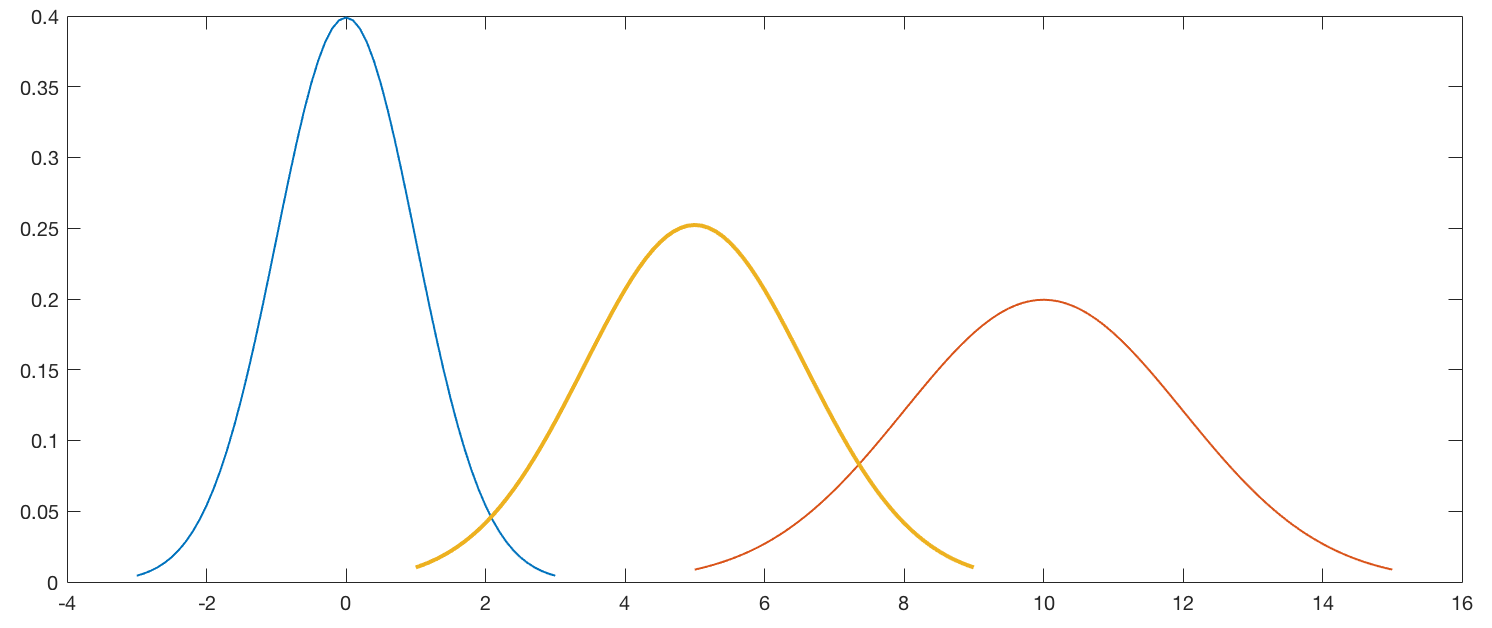
\includegraphics[width=1\linewidth]{Gaussian}
% 	\caption{Given two Gaussian probability measures $\N(0, 1)$ and $\N(10, 4)$, their displacement interpolation is $\N(10t, 1+3t)$ for any $t\in [0,1]$. The middle curve corresponds to the interpolation for $t=\frac{1}{2}$.}
% 	\label{fig:gaussian}
% \end{figure}

	
% It is known that \eqref{eq:wass-dist-defn} is a distance metric for two probability measures. In order to come up with a loss function for hypergraphs, one needs to define a measure of closeness among several probability measures. To this goal, we resort to Wasserstein barycenter \cite{Wasserstein_Barycenter}. The Wasserstein barycenter of $n$ probability measures $\mu_1,\cdots,\mu_n$ is defined as
% \begin{equation}
%     \label{eq:wass-barycenter}
% 	\mathsf{B}(\mu_1, \dots, \mu_n)\coloneqq \argmin_{\mu\in\mathcal{P}\left(L\right)}\sum_{i=1}^{n}\lambda_iW_p\left(\mu,\mu_i\right),
% \end{equation}
% where $\Lambda=(\lambda_1, \dots, \lambda_n)$ is a probability vector. It was established in \cite{CE2010} that, for $p=1$, the optimization problem \eqref{eq:wass-barycenter} is equivalent to the multi-marginal optimal transport problem
% \begin{equation*}
% 	\label{eq:mult-marginal-ot}
% 	\argmin_{\mu\in\Pi\left(\mu_1,\cdots,\mu_n\right)}\int_{L\times\cdots\times L}c\left(\xi_1,\cdots,\xi_n\right)\,\mathrm{d}\pi\left(\xi_1,\cdots,\xi_n\right)
% \end{equation*}
% where
% \begin{equation*}
% 	c\left(\xi_1,\cdots,\xi_n\right) = \inf_{x\in L}\sum_{i=1}^nd\left(\xi_i,x\right)
% \end{equation*}
% and $\Pi\left(\mu_1,\cdots,\mu_n\right)$ is the (convex) subset of probability distribution on $L\times\cdots\times L$ ($n$-copy Cartesian product) with marginal distribution $\mu_i$ on the $i$-th Cartesian component. This in turn demonstrates that \eqref{eq:wass-barycenter} is a linear program. The existence and uniqueness of Wasserstein barycenter is studied in \cite{Wasserstein_Barycenter}. In particular, it is shown that if $\mu_i=\N(m_i, \Sigma^2_i)$ for $i\in[n]\coloneqq \{1, \dots, n\}$ and if at least one of $\Sigma_i$ is full rank, then $\mathsf{B}(\mu_1, \dots, \mu_n) $ exists and is unique and equals $\N(m, \Sigma)$, where $m=\sum_i\lambda_im_i$ and $\Sigma$ is the unique solution of the fixed point equation $\Sigma = \sum_i\lambda_i(\Sigma^{1/2}\Sigma_i\Sigma^{1/2})^{1/2}$.  As indicated in \cite{Wasserstein_Barycenter}, Wasserstein barycenter extends displacement interpolation, allowing one to interpolate between several probability measures in a canonical way. Similar to \cite{Solomon:2014}, we motivate the use of Wasserstein barycenter as the loss function using the property of desired soft semi-supervised learning mentioned in \cite{Zhu:SSL_Gaussian}. It is shown in \cite[Theorem 3.6]{Barycenter_Variance} that 
% \begin{equation*}
%     \sum_{i=1}^{n}\lambda_iW_2\left(\mathsf{B}(\mu_1, \dots, \mu_n),\mu_i\right)\leq \sum_{i=1}^n\lambda_i \mathsf{var}(\mu_i),
% \end{equation*}
% where $\mathsf{var}(\cdot)$ denotes the variance of a given probability measure. Hence, if the variance of each $\mu_i$ are small, then their barycenter is concentrated within an intersection of small neighbourhoods around $\mu_i$.  
	
	
% \section{Hypergraph Label Propagation} \label{Sec:Label_propagat}
% Consider  a hypergraph $\H=(V, \cE)$ where $V=[n]$ and $\cE\subset 2^V$. Suppose we are given the soft labels $\mu_i\in \P(L)$ for a subset of vertices $i\in V_0$. For the ease of presentation, we assume $V_0=[k]$. The objective is to extend the labels to $\nu_1, \dots, \nu_n$ for all vertices in $V$ such that $\nu_i=\mu_i$ for all $i\in [k]$ and $\nu_i$ and $\nu_j$ are very "close" (in Wasserstein distance) if there exists $E\in \cE$ such that $i\in E$ and $j\in E$. For each $E\in \cE$, let $\mathsf{B}(E)$ be its \textit{centre of gravity} given by $\mathsf{B}(E)\coloneqq \mathsf{B}(\{\nu_j, j\in E\})$ where the $\lambda_i=\frac{1}{|E|}$. The goal is therefore written as 
% \begin{equation}
% 	\label{eq:wass-label-prop}
% 	\min_{\nu_1, \dots, \nu_n\in \P(L) \atop \nu_i=\mu_i, i\in [k]}\sum_{i=1}^m\eta_j\sum_{i\in E_j}W_2(\mathsf{B}(E_j), \nu_i),
% \end{equation}
% where $\eta_j$ is the weight of the $j$th hyperedge $E_j$(say $\frac{1}{|E_j|-1}$) and $m=|\cE|$. Clearly, the hard constraints $\nu_i=\mu_i$ for  $i\in [k]$ causes robustness issues. To avoid them, we propose the following objective function 
% \begin{equation}\label{eq:wass-label-prop-soft}
% 	\min_{\nu_1, \dots, \nu_n\in \P(L) }\sum_{i=1}^kW_2\left(\nu_i,\mu_i\right)+\sum_{j=1}^{m}\eta_j\sum_{i\in E_j}W_2(\mathsf{B}(E_j), \nu_i),
% \end{equation}    
% that is, the prescribed labels are to be reassigned "softly" through regularization rather than being hard-set. Given the definition of the centre of gravity, we can equivalently write the above optimization problem as follows: 
% \begin{equation}
% 	\label{eq:wass-label-prop-soft2}
%     \min_{\nu_1, \dots, \nu_n\in \P(L)}\min_{\zeta_1, \dots, \zeta_m\in \P(L)} \sum_{i=1}^kW_2\left(\nu_i,\mu_i\right)+\sum_{j=1}^{m}\eta_j\sum_{i\in E_j}W_2(\zeta_j, \nu_i).
% \end{equation}
% This double minimization allows us to apply the process of alternating minimization (aka Blahut-Arimoto algorithm \cite{Cover:2006}) to obtain the optimal labels $\nu_1, \dots, \nu_n$ which is described in sequel.
	

	
	
% %	
% %	{\color{red} POTENTIAL BULLSHIT: It seems to me that what matters is the number of labelled measures neighbors to each unlabelled measure, i.e., 
% %		$$\nu_j = \mathsf{bar}[\{\mu_r: \exists E\in \cE: r\in E, j\in E\}].$$ 
% %		The vertices whose neighbors are not labelled can be trivially assigned!!
% %		If this is not optimal, at least, this is the easiest assignment.
% %	}

% \subsection{Why not?}
% Address the computational cost? Dual formulation? Maybe use sink-horn or entropy regularization to speed up the distance calculation?  
	
% ******NEEDS TO BE COMPLETED****** 
	
	
% \section{Algorithm}\label{sec:algorithm}
% We propose to solve the optimization problem \eqref{eq:wass-label-prop-soft2} using an alternating minimization strategy. This amounts to two interleaved Wasserstein barycenter calculation.
	
% \emph{Step 0.} Initialize $\nu_i=\mu_i$ for $1\leq i\leq k$, and let $\nu_i$ be uniform distributions for all $k+1\leq i\leq n$.
	
% \emph{Step 1.} For fixed $\nu_1,\cdots,\nu_n$, compute $\mathsf{B}(E_1),\cdots,\mathsf{B}(E_m)$ for each of the $m$ hyperedges by
% \begin{equation}
% 	\label{eq:subproblem-barycenter}
% 	\mathsf{B}(E_j):=\frac{1}{|E_j|}\argmin_{\nu\in\mathcal{P}\left(L\right)}\sum_{i\in E_j}W_2\left(\nu, \nu_i\right).
% \end{equation}
	
% \emph{Step 2.} For fixed $\mathsf{B}(E_1),\cdots,\mathsf{B}(E_m)$, compute $\nu_1,\cdots,\nu_n$ for each of the $n$ vertices by  {\color{red}I think Step 3 needs to be edited. I wrote the objective as \eqref{eq:wass-label-prop} and changed it to \eqref{eq:wass-label-prop-soft} to make it look like previous works. If you don't agree with this way, let me know which one you like to keep, \eqref{eq:wass-label-prop} or \eqref{eq:wass-label-prop-soft}? }
% \begin{equation}
% 	\label{eq:subproblem-labels}
% 	\nu_i:=\argmin_{\nu\in\mathcal{P}\left(L\right)}\sum_{j:E_j\ni i}\eta_j W_2\left(\nu_j^b, \nu\right)
% \end{equation}
% and then set
% \begin{equation*}
% 	\nu_i=\mu_i\quad\textrm{for all $1\leq i\leq k$}.
% \end{equation*}
	
% \emph{Step 3.} Repeat Step 1-2 until convergence, or until a predetermined number of iterations is reached.
	
% %	{\color{blue} @Yi: This is really just a preliminary version of the algorithm. I think this version might need some tweaking to be made to work --- maybe by a change of the iteration order (e.g. randomly initializing the barycenters first), or using dynamically adaptive weights, or it might only work for particular Wasserstein distances ($p=1$ or $p=2$?), or the barycenter application should be replaced with a version with entropy regularization... I think it really depends on experiments!}
% %	
% %	{\color{red} @Tingran: When we assume the probabilities are supported on the classes, I use the python optimal transport (ot) package, and the barycenter and Wasserstein distances are in $W_1$ and entropy regularized ($\text{reg}=0.01$), but in the case of Gaussian, the closed form in literature is in $W_2$, if I understood it correctly. The code I have now initializes vertex probabilities randomly, but it is not a big deal that I do the other way around. I don't quite understand what do you mean by ``dynamically adaptive weights'', so would you please offer more details about it?}
% %	
% %	{\color{blue} Of course! I was thinking about updating the weights $\eta_j$ during the iteration as well, for instance, one can set $\eta_j$ to be proportional to the weighted degree of the hyperedge. But it is probably tricky to get it right in implementation (the update rule will be crucial for convergence), so we don't have to do it right now --- it was just an idea that ran across my mind.}
% %	


% \subsection{Convergence:}
% If all known labels have the same variances, then the variance of each unknown labels converge to that of known ones. *******[Needs proof]********* 

% \section{Linear Hypergraphs}
% Suppose that $H$ is a \textit{linear} hypergraph, that is every two hyperedges of $H$ have at most one vertex in common and each vertex is contained in at most two hyperedges. Suppose also that from each hyperedge, we observe the label of exactly one vertex, thus $k=m$. 
	
% Recall that we assume that the labels $\{\mu_i\}_{i=1}^k$ are given for the vertices $i\in\{k\}$ and the objective is to derive the appropriate labels for vertices $j\in \{k+1, \dots, n\}$. In first case, we assume that the labels are given for all vertices of degree two. Consider the hyperedge $E$ with $r$ vertices of degree two with labels, say, $\mu_1, \dots, \mu_r$. It is clear that the optimal labels for the rest of vertices in $E$ are $\mathsf{B}(\mu_1, \dots, \mu_r)$. The more interesting case is when the degree of all labelled vertices are one. Let $\Xi(E)\coloneqq -|E| + \sum_{i\in E}d_i$. In fact, $\Xi(E)$ specifies the number of hyperedges that are incident to $E$, this it may be well called the \textit{conductivity} of $E$. We shall show that with the above assumption, the optimal labels are obtain via the following simple rules [Needs to be verified]:
% \begin{itemize}
% 	\item $\nu_i = \mu_r$ if $d(i)=1$ and $(i, r)\in E$ for some $E\in \cE$ and $r\in [k]$
% 	\item $\nu_i = \mu_r$ if $d(i)=2$ and $(i, j)\in E_1$ and $(i, r)\in E_2$ with $\Xi(E_2)>\Xi(E_1)$ for some $j\in [k]$
% 	\item $\nu_i = [\mu_r, \mu_j]_t$ if $d(i)=2$ and $(i, j)\in E_1$ and $(i, r)\in E_2$ with $\Xi(E_2) = \Xi(E_1)$ for some $r, j\in [k]$ and $t\in [0,1]$.   
% \end{itemize}
% *****NEEDS TO BE COMPLETED******
	
	

	

	
% \section{Experiments}
% \subsection{Binary classification}
% \subsection{Regression}

	
	
	
\bibliography{bibliography}
  \bibliographystyle{aaai}	

\end{document}

